\documentclass[12pt]{article}
\usepackage{verbatim}
\usepackage[dvips]{epsfig}
\usepackage{color}
\usepackage{url}
\usepackage[colorlinks=true]{hyperref}

\begin{document}

\section*{GENESIS: Documentation}

{\bf Related Documentation:}
% start: userdocs-tag-replace-items related-do-nothing
% end: userdocs-tag-replace-items related-do-nothing

\section*{De Schutter: Purkinje Cell Model}

\begin{figure}[h]
\centering
   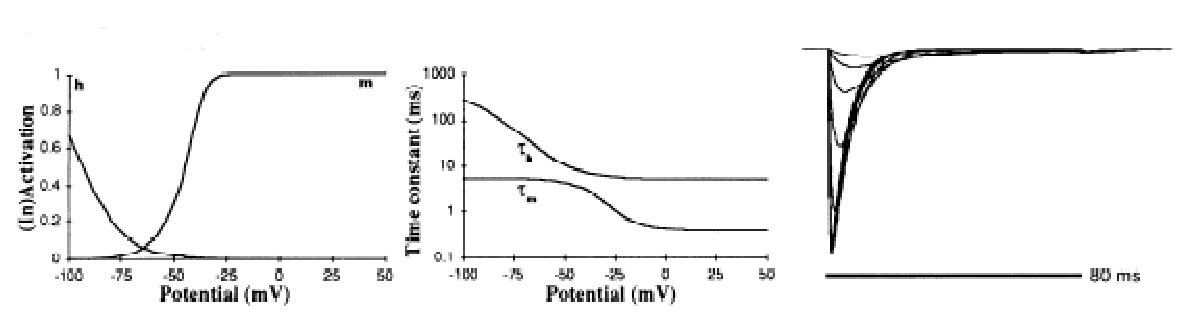
\includegraphics[scale=0.75]{figures/DS1.2B.eps}
   \caption{Activation and inactivation properties of the T-type calcium current (CaT, ---) in the model. Seady-state activation and inactivation vs. voltage are plotted at the {\em left}, the time constants of activation ($\tau_m$) and inactivation ($\tau_h$) vs. voltage in the {\em middle} (Note: Semilogarithmic scale), and a simulation of representative voltage-clamp currents at the {\em right}.}
   \label{fig:DS1.2B}
\end{figure}

\subsection*{T-Type Calcium Current}

Several groups have reported the presence of a low-threshold, inactivating Ca$^{2+}$ channel in the Purkinje
cell\,\cite{Gruol:1990vn, Hirano:1989uq, Kaneda:1990ys} comparable to the T channel in other neurons\,\cite{Fox:1987zr}. The whole-cell voltage-clamp study of freshly isolated rat Purkinje cells by \,\cite{Kaneda:1990ys} (their Figs. 1--3) provided all the data necessary to model activation of T calcium (CaT) current (Fig. 2 B). \,\cite{Hirano:1989uq} (their Fig. 4$C$) have shown a higher threshold of activation for CaT current in Purkinje cells, but\,\cite{Gruol:1990vn} reported the same threshold as\,\cite{Kaneda:1990ys}. The equations for CaT current inactivation were based on a combination of steady-state inactivation data from\,\cite{Hirano:1989uq} (their Fig. 5$A$) and time constant data from\,\cite{Kaneda:1990ys} (their Fig. 2$B$), which were almost identical to the data from\,\cite{Hirano:1989uq} (their Fig. 5$C$).

\bibliographystyle{plain}
\bibliography{../tex/bib/g3-refs}

\end{document}
